\section{Experiments}
\subsection{Case Studies}
We design and impltement a web-based interface to demonstrate our cases~\footnote{}.
All cases are available in our website~\footnote{}.

\subsubsection{IMDb movies}\label{sec:imdb_movies}
We first introduce a simple case with the IMDb movie dataset~\cite{} (Figure~\ref{fig:iMDBMovies}).

% 我们挑选了数据集中2019年在中国上映的电影。
\textbf{Graph Wrangling}. We select movies in the dataset which is published in 2019 and is released in China.
% 我们保留了其中标题、发布日期、演员、类别、
We preserve seven attributes for movies: title, the publish date (\texttt{"date\_published"}), actors, genre, director, writer, and country.
Two movies are connected if they share at least one same actor.
We generate an attribute, \texttt{"shared\_actors"}, for each link. 
It records the number of shared actors.
We totally obtain 49 nodes and 99 links.

\textbf{Visual Encoding}. Nodes are visualized as \texttt{<circle>}s and links are visualized as \texttt{<line>}s.
The fill colors of \texttt{<circle>}s encode their publish seasons.
The width of \texttt{<line>}s encode the \texttt{"shared\_actors"}.

\textbf{Layout}. We pre-compute a layout with a spring layout algorithm~\cite{DBLP:journals/spe/FruchtermanR91}.
Our approach generate descriptions for it:
\begin{compactitem}
    \item \textbf{Linking Condition}. Two nodes are connected if their attributes \colorbox{text-highlight}{\color{white}actors} share an intersection.
    \item \textbf{Visual Encoding}.
    \begin{compactitem}
        \item Each node consists of only 1 primitive.
        \item It is a \texttt{<circle>}. 
        \item Its fill encodes the attribute date\_published@month.
        \begin{compactitem}
            \item When the value of the attribute date\_published@month is 04, 06, or 05, its fill turns to \#ff7f0e.
            \item When the value of the attribute date\_published@month is 10, 12, or 11, its fill turns to \#d62728.
            \item When the value of the attribute date\_published@month is 09, 07, or 08, its fill turns to \#2ca02c.
            \item When the value of the attribute date\_published@month is 03, 02, or 01, its fill turns to \#1f77b4.
        \end{compactitem}
        \item Each link consists of only 1 primitive.
        \item It is a \texttt{<line>}.
        \item Its stroke-width encodes the attribute shared\_actors.
            The greater the shared\_actors is, the greater its stroke-width is.
    \end{compactitem}
    \item \textbf{Layout Condition}. 
\end{compactitem}

The descriptions are generated as expected.
Whereas, our technique does not detect that the color of each node encodes the published season because ``season'' is not included in attributes of nodes.
However, it generates the mapping of different color categories, such that audience can obtain that the fill color encodes the ``season''.

\begin{figure}
    \centering
    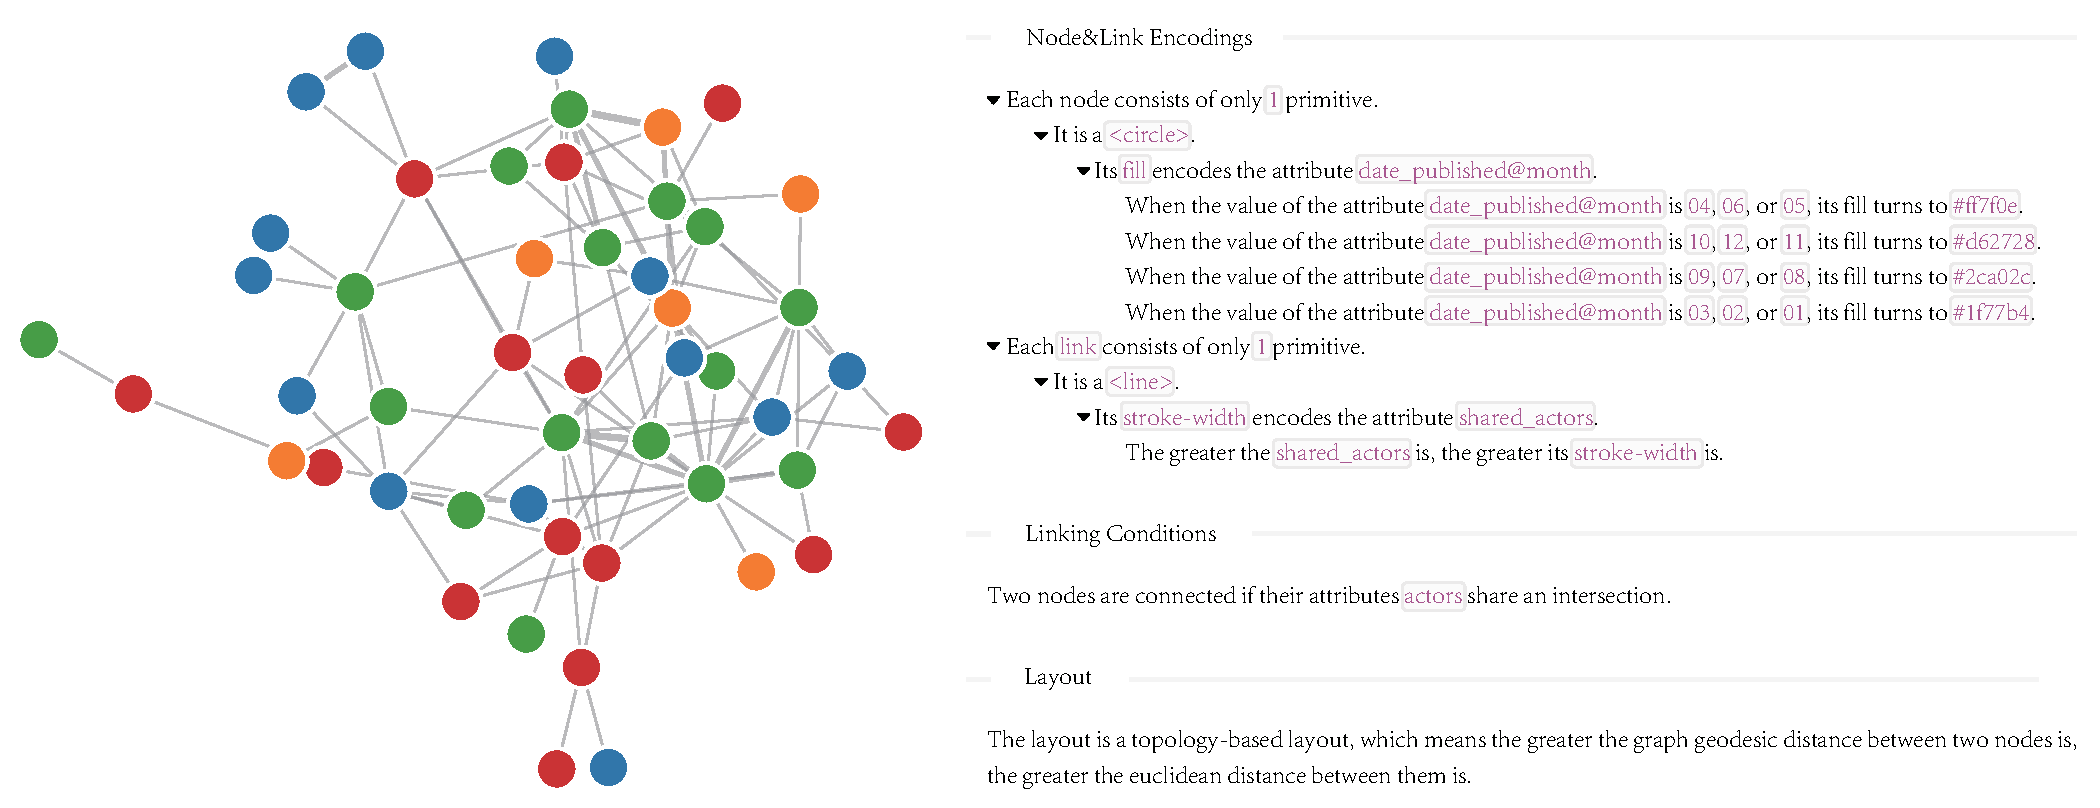
\includegraphics[width=1\columnwidth]{figures/iMDBMovies.eps}
    \caption{xxx}
    \label{fig:iMDBMovies}
\end{figure}


\subsubsection{IMDb actors}
With the IMDb movie dataset in Case~\ref{sec:imdb_movies}, we introduce another case which focuses on actors.

\textbf{Graph Wrangling}. We first select movies in the dataset that are only released in China from 2016 to 2021.
Their actors who have acted in more than five movies are regarded as nodes.
Each actor has five attributes: name, movies (s/he acted in from 2016 to 2021), the average vote (\texttt{"avg\_vote"}), the number of votes s/he got (\texttt{"votes"}), the number of movies in each year from 2016 to 2021 (\texttt{"number\_of\_movies\_by\_year"}).
Two actors are connected if they acted in at least one movie from 2016 to 2021.
We preserve the number of movies (\texttt{"number\_of\_shared\_movies"}) they both acted in in the link.

\textbf{Visual Encoding}. To show the activeness of each actor, we embed a simple line chart for each node to show the number of movies s/he acted in from 2016 to 2021. Similar to Case~\ref{sec:imdb_movies}, The width of \texttt{<line>}s encode its attribute \texttt{"number\_of\_shared\_movies"}.

\textbf{Layout}. We utilize the layout to show two attributes (\texttt{"avg\_vote"} and \texttt{"votes"}) of each node. The x-coordinate encodes the attribute \texttt{"votes"} and the y-coordinate encodes the \texttt{"avg\_vote"}.

Different with Case~\ref{sec:imdb_movies}, in this case, each node consists of several primitives.
We distinguish primitives into different entities and classify primitives of one data entity into different roles.
We interpret the meaning of the line chart by describing its primitives (\texttt{<line>}s).

\subsubsection{}

\subsubsection{Failure Cases}

\subsection{User Studies}
第一部分,找一些创作者,让他们阅读代码,为代码和节点链接图生成相应的描述;
通过让他们自己比较自己生成的描述和自动生成的描述,为描述进行打分。

第二部分,找一些不懂图可视化的人,让他们看生成的描述,回答一些问题。